

\tikzset{every picture/.style={line width=0.75pt}} %set default line width to 0.75pt        

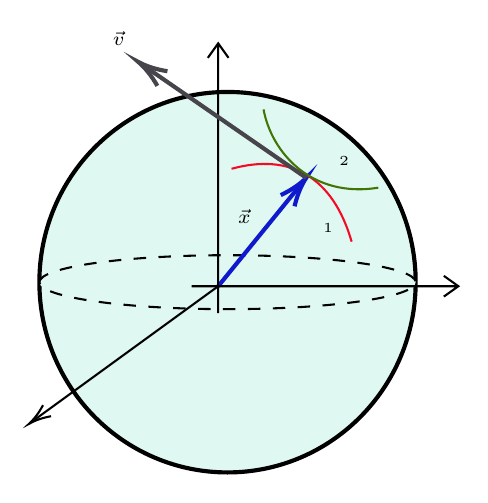
\begin{tikzpicture}[x=0.75pt,y=0.75pt,yscale=-1,xscale=1]
%uncomment if require: \path (0,300); %set diagram left start at 0, and has height of 300

%Shape: Ellipse [id:dp8621922183495604] 
\draw  [fill={rgb, 255:red, 223; green, 248; blue, 241 }  ,fill opacity=1 ][line width=1.5]  (171.14,159.71) .. controls (171.14,109.08) and (211.73,68.05) .. (261.79,68.05) .. controls (311.85,68.05) and (352.43,109.08) .. (352.43,159.71) .. controls (352.43,210.33) and (311.85,251.37) .. (261.79,251.37) .. controls (211.73,251.37) and (171.14,210.33) .. (171.14,159.71) -- cycle ;
%Shape: Ellipse [id:dp2859403935407516] 
\draw  [fill={rgb, 255:red, 223; green, 248; blue, 241 }  ,fill opacity=1 ][dash pattern={on 4.5pt off 4.5pt}] (171.14,159.71) .. controls (171.14,152.53) and (211.73,146.71) .. (261.79,146.71) .. controls (311.85,146.71) and (352.43,152.53) .. (352.43,159.71) .. controls (352.43,166.89) and (311.85,172.71) .. (261.79,172.71) .. controls (211.73,172.71) and (171.14,166.89) .. (171.14,159.71) -- cycle ;
%Straight Lines [id:da16269634334020433] 
\draw [color={rgb, 255:red, 15; green, 26; blue, 204 }  ,draw opacity=1 ][line width=1.5]    (257.29,161.66) -- (297.82,111.76) ;
\draw [shift={(299.71,109.43)}, rotate = 129.09] [color={rgb, 255:red, 15; green, 26; blue, 204 }  ,draw opacity=1 ][line width=1.5]    (14.21,-4.28) .. controls (9.04,-1.82) and (4.3,-0.39) .. (0,0) .. controls (4.3,0.39) and (9.04,1.82) .. (14.21,4.28)   ;
%Shape: Axis 2D [id:dp5781161322417953] 
\draw  (244.43,161.66) -- (373,161.66)(257.29,44.64) -- (257.29,174.66) (366,156.66) -- (373,161.66) -- (366,166.66) (252.29,51.64) -- (257.29,44.64) -- (262.29,51.64)  ;
%Straight Lines [id:da986530720222472] 
\draw    (257.29,161.66) -- (167.62,226.87) ;
\draw [shift={(166,228.05)}, rotate = 323.97] [color={rgb, 255:red, 0; green, 0; blue, 0 }  ][line width=0.75]    (10.93,-3.29) .. controls (6.95,-1.4) and (3.31,-0.3) .. (0,0) .. controls (3.31,0.3) and (6.95,1.4) .. (10.93,3.29)   ;
%Curve Lines [id:da2567673398245671] 
\draw [color={rgb, 255:red, 245; green, 10; blue, 38 }  ,draw opacity=1 ]   (263.71,105.08) .. controls (292,97.28) and (312.57,108.98) .. (321.57,140.18) ;
%Curve Lines [id:da2661789837245453] 
\draw [color={rgb, 255:red, 65; green, 117; blue, 5 }  ,draw opacity=1 ]   (279.14,76.48) .. controls (283,97.28) and (302.29,119.38) .. (334.43,114.18) ;
%Straight Lines [id:da53165768173298] 
\draw [color={rgb, 255:red, 71; green, 68; blue, 75 }  ,draw opacity=1 ][fill={rgb, 255:red, 61; green, 57; blue, 57 }  ,fill opacity=1 ][line width=1.5]    (299.71,109.43) -- (221.18,55.23) ;
\draw [shift={(218.71,53.53)}, rotate = 34.61] [color={rgb, 255:red, 71; green, 68; blue, 75 }  ,draw opacity=1 ][line width=1.5]    (14.21,-4.28) .. controls (9.04,-1.82) and (4.3,-0.39) .. (0,0) .. controls (4.3,0.39) and (9.04,1.82) .. (14.21,4.28)   ;

% Text Node
\draw (265.43,123.4) node [anchor=north west][inner sep=0.75pt]  [font=\scriptsize]  {$\vec{x}$};
% Text Node
\draw (205,37.59) node [anchor=north west][inner sep=0.75pt]  [font=\scriptsize]  {$\vec{v}$};
% Text Node
\draw (306.43,130.05) node [anchor=north west][inner sep=0.75pt]  [font=\scriptsize]  {$\upsigma _{1} \ \ $};
% Text Node
\draw (314.14,97.55) node [anchor=north west][inner sep=0.75pt]  [font=\scriptsize]  {$\upsigma _{2} \ \ $};


\end{tikzpicture}
